\section{Entwurf auf Geschäftsprozessebene}\label{sec:modellierung}
Die Fertigungsdurchführung in der diskreten Fertigung basiert derzeit, wie in Kapitel \ref{ch:Bezugsrahmen} erläutert, auf einem statischen und ablauforientierten Geschäftsprozess der durch SAP S/4HANA Cloud abgebildet werden kann. Der Geschäftsprozess wird anhand der, in Abbildung \ref{fig:Typische Prozessschritte der Fertigungsdurchführung} illustrierten, typischen Prozessschritte der Fertigungsdurchführung, sowie deren Merkmale und Defizite charakterisiert. Die Anforderungen die es im Rahmen der vorliegenden Bachelorarbeit umzusetzen gilt, werden in Abschnitt \ref{sec:anforderungen} zusammengetragen.

Für die Entwicklung geeigneter Maßnahmen zur Erfüllung der Anforderungen, werden die Merkmale und Defizite der Fertigungsdurchführung unter Einbeziehung der Leitgedanken von Lean Management betrachtet. Die Maßnahmen haben das Ziel, den Geschäftsprozess möglichst dynamisch und ereignisorientiert abzubilden.

Durch die Modellierung von Dynamikeinheiten sollen die wesentlichen Zusammenhänge in den Prozessschritten der Fertigungsdurchführung dargestellt werden. Da \ac{BPMN} 2.0 für die Modellierung des Geschäftsprozesses zum Einsatz kommt, werden zur Bildung einer Dynamikeinheit die in Tabelle \ref{tab:dynmaikelemente} genannten Symbole verwendet.

\begin{table}[H]
	\centering
	\begin{tabularx}{\textwidth}{l c X} 
		\toprule
		\textbf{Element}  &  
		\textbf{BPMN-Symbol} &
		\textbf{Beschreibung}  \\ 
		\midrule
		
		Auslöser &   
		\begin{minipage}{.1\textwidth}
            
\includegraphics[width=\linewidth]{img/startevent.png}
        \end{minipage}  &
		 Initiierendes Ereignis         \\  \cmidrule(r){1-1} \cmidrule(r){2-2} \cmidrule(r){3-3}
		
		Aktivität &   
		\begin{minipage}{.2\textwidth}
            
\includegraphics[width=\linewidth]{img/service.png}
        \end{minipage}  &
		Dienstaufgabe, wird von einem digitalisierten Dienst automatisch ausgeführt \cite{OMG.2014}        \\   \cmidrule(r){2-2} \cmidrule(r){3-3}
		
		 &   
		\begin{minipage}{.2\textwidth}
            
\includegraphics[width=\linewidth]{img/user.png}
        \end{minipage}  &
		Benutzeraufgabe, wird vom Anwender manuell und mit \ac{IT}-Unterstützung ausgeführt        \\   \cmidrule(r){2-2} \cmidrule(r){3-3}
		
		 &   
		\begin{minipage}{.2\textwidth}
            
\includegraphics[width=\linewidth]{img/manual.png}
        \end{minipage}  &
		Manuelle Aufgabe, wird vom Anwender manuell und ohne \ac{IT}-Unterstützung ausgeführt        \\  \cmidrule(r){2-2} \cmidrule(r){3-3}
		
				 &   
		\begin{minipage}{.2\textwidth}
            
\includegraphics[width=\linewidth]{img/subprocess.png}
        \end{minipage}  &
		Teilprozess, wird in einem zugehörigen Teilprozessmodell detailierter beschrieben        \\  \cmidrule(r){1-1} \cmidrule(r){2-2} \cmidrule(r){3-3}
		
		Resultat &   
		\begin{minipage}{.1\textwidth}
            
\includegraphics[width=\linewidth]{img/endevent.png}
        \end{minipage}  &
		Ausgelöstes Ereignis  \\
	    \bottomrule
	\end{tabularx}
	\caption{\label{tab:dynmaikelemente}Elemente in einer Dynamikeinheit}
\end{table}

Bei der Entwicklung dynamischer Geschäftsprozessmodelle in \ac{BPMN} 2.0 müssen anschließend die Verknüpfungen zwischen den Dynamikeinheiten spezifiziert werden, da sie verantwortlich für einen korrekten Geschäftsprozessablauf sind. 
Diese betrachtet verschiedene Askpekte und Regeln, mit denen primär ablauforientierte Geschäftsprozesse aus der Realität durch Software abgebildet werden. Die wesentlichen Betrachtungen in diesem Bezug sind der Aufruf digitaler Dienste, die technische Anbindung von manuellen Benutzeraufgaben und die Behandlung von Ereignissen im Geschäftsprozess.

\newpage

\subsection{Vorstellung der ausgewählten Maßnahmen}
Die ausgewählten Maßnahmen zur Dynamisierung der existierenden Fertigungsdurchführung in SAP S/4HANA Cloud werden zunächst im Folgenden einzeln dargestellt und erörtert.

\paragraph{Maßnahme 1: Freigabe des Fertigungsauftrags ($\rightarrow$ \textbf{ANF-1})}
Ein häufig erwähntes Merkmal für die Entwicklung dynamischer Geschäftsprozesse ist die Notwendigkeit einer flexiblen und effizienten Ablaufplanung. In der Praxis wird die Fertigungsdurchführung mit SAP S/4HANA Cloud in der Regel nur mithilfe eines Medienbruchs realisiert. Ein vollständiger digitaler Informationsfluss in der Fertigungsrückmeldung ist in der Realität keine gängige Methode und die meisten Industriebetriebe sind derzeit noch nicht in der Lage auf eine papierlose Produktion umzusteigen.

Betrachtet man diesen Zustand unter Einbeziehung der Leitgedanken von Lean Management wird schnell klar, dass in diesem Schritt durch den Austausch von Informationen in Papierform Verschwendung von Zeit und Ressourcen entsteht. Um dieser Problemstellung entgegenzutreten schlägt der Autor der vorliegenden Bachelorarbeit einen hybriden Ansatz zur Problemlösung vor.

Ein Ereignis soll bei der Freigabe eines Fertigungsauftrages in Echtzeit ausgelöst werden. Auf der Grundlage dieses Ereignisses soll der zuständige Werker digital über ein mobiles Gerät benachrichtigt werden
($\rightarrow$ \textbf{ANF-4}).
Dieser kann nun entscheiden, ob die Informationen in der mobilen Anwendung ausreichend sind oder ob er sie lieber ausdruckt. Der Vorteil hierbei ist, dass der Werker unmittelbar über eine Aktualisierung seines Arbeitsvorrats Bescheid weiß und ohne Zeit durch unnötige Laufwege, wie die Abholung der Fertigungsaufträge beim Fertigungssteuerer, zu verschwenden, mit der Abarbeitung der Fertigungsaufträge beginnen kann. Durch den Einsatz von mobilen Anwendungen, die über offene Schnittstellen mit SAP S/4HANA Cloud kommunizieren, können stationäre Terminals in den Werken überflüssig gemacht werden und Verschwendungen in Form von Latenzen können vermieden werden.

\paragraph{Maßnahme 2: Rückmeldung des Fertigungsauftrags ($\rightarrow$ \textbf{ANF-2})}
Die Gegebenheiten des Produktionsfortschritts werden durch Rückmeldungen der einzelnen Fertigungsaufträge ermittelt. Eine Rückmeldung ist ein Teil der Betriebsdatenerfassung. Sie dokumentiert den Stand der Bearbeitung, von Vorgängen, sowie Material- und Zeitverbräuche. Im SAP S/4HANA Cloud unterscheidet man zwischen Teilrückmeldung und Endrückmeldung. 

Die Erfassung der Rückmeldung wird in der Regel auf Papier oder an einem Terminal durchgeführt. Da diese Ansätze beide in die Kategorien von Verschwendung im Sinne von Lean Management fallen, sollen sie vermieden werden.
Auch hier wird, aufgrund der Notwendigkeit der Unterstützung einer papierbasierten Produktion, ein hybrider Ansatz zur Problemlösung verfolgt.

Die Erfassung der Rückmeldung wird demnach in zwei Ausführungen unterstützt. Der erste Ansatz stellt die Rückmeldung der Betriebsdaten durch den ausschließlichen Einsatz von mobilen Geräten dar
($\rightarrow$ \textbf{ANF-4}).
Die Nutzenaspekte einer mobilen Anwendung lassen sich einfach anhand der eingesparten Prozessschritte erklären.
Denn eine vollständige, digitale Umsetzung der Betriebsdatenerfassung in der Fertigungsdurchführung macht Laufwege zu Terminals, den Druck von Arbeitspapieren und die doppelte Datenerfassung überflüssig.
Parallel dazu wird die Möglichkeit angeboten, weiterhin auf Papier zu arbeiten. Zur Verkürzung der Durchlaufszeiten soll die Eingabe der Betriebsdaten jedoch nicht manuell in S/4HANA Cloud erfolgen, sondern durch das Scannen des Rückmeldescheins in Papierform. Hierfür wird mit einem mobilen Gerät lediglich ein Foto des Rückmeldescheins gemacht, der Text wird erkannt, die erkannten Daten werden wiederum vom Werker bestätigt und anschließend über eine Schnittstelle zu SAP S/4HANA Cloud erfasst.

\paragraph{Maßnahme 3: Erfassung von Defekten ($\rightarrow$ \textbf{ANF-3})}
Im Bereich der Kontrolle und Steuerung der Fertigungsdurchführung ist es wichtig zu erfahren, ob Ausschuss produziert wurde oder Nacharbeit entstanden ist. Ausschuss ist der Anteil der Produkte, der nicht den Qualitätsanforderungen entspricht.
Nacharbeit ist die Beseitigung von Fehlern an Erzeugnissen des Industriebetriebes.
Beim ersten Auftreten eines solchen Qualitätsmangels, aber auch bei sonstigen Hindernissen, die Einfluss auf die Fertigungsdurchführung haben, sollten umgehend Defekte gemeldet werden.



Defekte werden in der Regel persönlich an den Fertigungssteuerer berichtet oder an einem Terminal durchgeführt. Beide Ansätze können keine unmittelbare Erfassung gewährleisten und entsprechen somit nicht den Anforderungen eines Echtzeitunternehzmens.
Der Autor verfolgt hierbei einen digitalen Ansatz zur Problemlösung.

Die Erfassung von Defekten soll demnach durch den Einsatz von mobilen Geräten unterstützt werden
($\rightarrow$ \textbf{ANF-4}).
Eine Erfassung von Defekten in Echtzeit macht es möglich unmittelbar auf sie zu reagieren, um so potenzielle Verschwendungen zu eliminieren.

\subsection{Segmentierung und Bildung von Dynamikeinheiten}
Nach der Erarbeitung der fachlichen Maßnahmen werden die Aktivitäten der Fertigungsdurchführung zur Dynamisierung mittels Segmentierung und Bildung von Dynamikeinheiten in Wechselwirkung mit Ereignissen gesetzt. 
(siehe auch \citeauthor{Alexopoulou.2008} \cite{Alexopoulou.2008} und \citeauthor{Vidackovic.2014} \cite{Vidackovic.2014}) 

Die Geschäftsprozessebene muss hinreichend dynamisch sein, um den Ablauf der Fertigungsdurchführung als Reaktion auf relevante Ereignisse aus der Ereignisverarbeitungsebene betrachten zu können. 
Bei der Segmentierung der Fertigungsdurchführung in Aktivitäten werden daher folgende Merkmale beachtet:
\begin{itemize}
    \item Als Aktivität ist entweder ein Aufruf eines digitalen Dienstes, eine Benutzeraufgabe mit \ac{IT}-Unterstützung, eine manuelle Aufgabe ohne \ac{IT}-Unterstützung oder aber ein Teilprozess als Verdichtung weiterer Aktivitäten anzusehen.
    \item Den Auslöser einer Aktivität stellt immer ein oder mehrere initiierende Ereignisse dar.  Demnach erfolgt die Ausführung einer Aktivität nur bei Auftreten dieses Ereignisses, wohingegen dessen Ausbleiben dynamisch zu einem anderen Ablauf des Geschäftsprozesses führt.
    \item Eine Aktivität löst nach ihrer Durchführung ein oder mehrere Folgeereignisse aus, die für den weiterführenden Ablauf des Geschäftsprozesses führen.
\end{itemize}

Das Ereignis \textit{\enquote{Fertigungsauftrag freigeben}} stellt dabei den Auslöser zur Benachrichtigung des Werkers dar (siehe Abbildung \ref{fig:Dynamikeinheit zur Benachrichtigung des Werkers}). Hierbei wird der Werker in Echtzeit über einen neuen Fertigungsauftrag unterrichtet. Nach dem Abschluss der Benachrichtigung wird das Ereignis \textit{\enquote{Fertigungsauftrag empfangen}} ausgelöst.

\begin{figure}[H]
	\centering 
    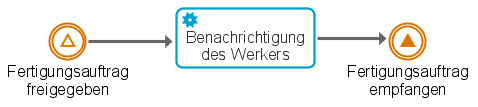
\includegraphics[width=.7\textwidth]{img/freigabeeinheit.png}	
    \caption[Dynamikeinheit zur Benachrichtigung des Werkers]
    {Dynamikeinheit zur Benachrichtigung des Werkers\protect\footnotemark}
    \label{fig:Dynamikeinheit zur Benachrichtigung des Werkers}
\end{figure}
\footnotetext{Eigene Darstellung}

Die Dynamikeinheit zur Auftragsabarbeitung wird durch das Ereignis \textit{\enquote{Fertigungsauftrag empfangen}} oder aber durch eine Teilrückmeldung angestoßen (siehe Abbildung \ref{fig:Dynamikeinheit zur Auftragsabarbeitung}). Sobald in der Auftragsabarbeitung relevante Fortschritte zu verzeichnen sind, wird das Ereignis \textit{\enquote{Fertigungsauftrag fortgeschritten}} ausgelöst.

\begin{figure}[H]
	\centering 
    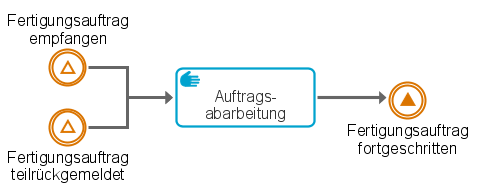
\includegraphics[width=.7\textwidth]{img/abarbeitungseinheit.png}	
    \caption[Dynamikeinheit zur Auftragsabarbeitung]
    {Dynamikeinheit zur Auftragsabarbeitung\protect\footnotemark}
    \label{fig:Dynamikeinheit zur Auftragsabarbeitung}
\end{figure}
\footnotetext{Eigene Darstellung}

Das Ereignis \textit{\enquote{Fertigungsauftrag fortgeschritten}} ist der Auslöser für zwei weitere Aktivitäten.
Zum einen wird die Erfassung der Betriebsdaten in Form von Rückmeldungen angestoßen, die als Folge eine Teilrückmeldung oder eine finale Rückmeldung haben kann (siehe Abbildung \ref{fig:Dynamikeinheit zur Rückmeldung}).

\begin{figure}[H]
	\centering 
    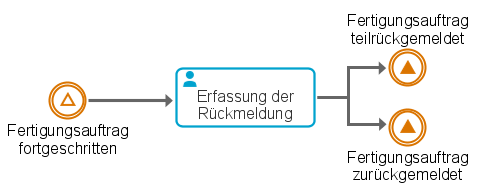
\includegraphics[width=.7\textwidth]{img/ruckmeldeeinheit.png}	
    \caption[Dynamikeinheit zur Rückmeldung]
    {Dynamikeinheit zur Rückmeldung\protect\footnotemark}
    \label{fig:Dynamikeinheit zur Rückmeldung}
\end{figure}
\footnotetext{Eigene Darstellung}

Auf Anderen wird zur selben Zeit eine Qualitätsprüfung ausgelöst. Diese kann als Ergebnis ein positives Ereignis \textit{\enquote{Qualität fehlerfrei}} oder ein negatives Ereignis \textit{\enquote{Qualität fehlerhaft}} nach sich ziehen (siehe Abbildung \ref{fig:Dynamikeinheit zur Qualitätsprüfung}).

\begin{figure}[H]
	\centering 
    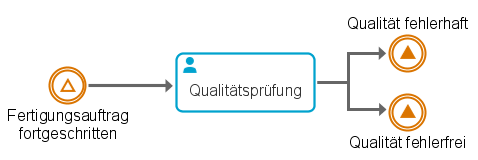
\includegraphics[width=.7\textwidth]{img/qualiit.png}	
    \caption[Dynamikeinheit zur Qualitätsprüfung]
    {Dynamikeinheit zur Qualitätsprüfung\protect\footnotemark}
    \label{fig:Dynamikeinheit zur Qualitätsprüfung}
\end{figure}
\footnotetext{Eigene Darstellung}

Eine jede Erfassung von Betriebsdaten wird dabei auf Plausibilität überprüft. Sind die Eingaben fehlerfrei, wird diese Dynamikeinheit keinen Einfluss auf den weiteren Ablauf der Fertigungsdurchführung nehmen (siehe Abbildung \ref{fig:Dynamikeinheit zur Plausibilitätsprüfung}).
Bei fehlerhaften Betriebsdaten folgt jedoch das Ereignis \textit{\enquote{Betriebsdaten fehlerhaft}}.

\begin{figure}[H]
	\centering 
    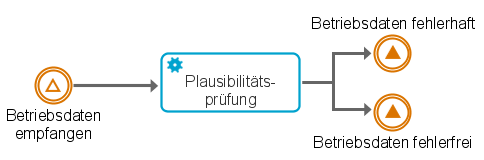
\includegraphics[width=.7\textwidth]{img/plausibilit.png}	
    \caption[Dynamikeinheit zur Plausibilitätsprüfung]
    {Dynamikeinheit zur Plausibilitätsprüfung\protect\footnotemark}
    \label{fig:Dynamikeinheit zur Plausibilitätsprüfung}
\end{figure}
\footnotetext{Eigene Darstellung}

Im Falle, dass während der Fertigungsdurchführung ein Problem mit der Daten- oder Produktqualität auftritt, muss ein Defekt erfasst werden(siehe Abbildung \ref{fig:Dynamikeinheit zur Erfassung von Defekten}). Dieser kann in der Produktionsplanung- und steuerung dann analysiert und bewertet werden.

\begin{figure}[H]
	\centering 
    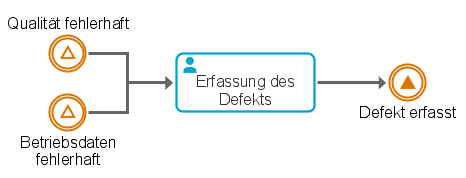
\includegraphics[width=.7\textwidth]{img/defectiit.png}	
    \caption[Dynamikeinheit zur Erfassung von Defekten]
    {Dynamikeinheit zur Erfassung von Defekten\protect\footnotemark}
    \label{fig:Dynamikeinheit zur Erfassung von Defekten}
\end{figure}
\footnotetext{Eigene Darstellung}

% \subsection{Aspekte der Ausführungssemantik}

% \missingfigure{ Wesentliche Aspekte der Ausführungssemantik}